\documentclass[12pt]{article}

\usepackage{sbc-template}
\usepackage{graphicx,url}
\usepackage[brazil]{babel}   
%\usepackage[latin1]{inputenc}  
\usepackage[utf8]{inputenc}
% professional-quality tables
\usepackage{booktabs}
% Pacote para gerenciamento de flutuantes, como iamgens e tabelas.
\usepackage{float}
% Biblioteca para quebrar linhas em células de tabelas
\usepackage{makecell}
% UTF-8 encoding is recommended by ShareLaTex
     
\sloppy
\title{Sistemas de Gerenciamento de Biblioteca:\\ Um Mapeamento Sistemático}
\author{Evelyn G. de Oliveira Santos\inst{1}, Felipe N. Guedes\inst{1}, Luiz Felipe da C. Souza\inst{1},\\ Ricardo J. P. Salgueiro\inst{1}, Felipe F. de Souza\inst{1}}
\address{Departamento de Computação -- Universidade Federal de Sergipe
  (UFS)\\Av. Marechal Rondon, Rosa Elze -- 49.100-00 -- São Cristóvão -- SE -- Brazil
  \email{evelyngabill96@gmail.com, tututs0@hotmail.com}
  \emailnew{luizfcs@dcomp.ufs.br, salgueiro@ufs.br}% esse comando foi criado dentro do arquivo .sty mas pode trazer para este arquivo se desejar
  }
\begin{document} 

\maketitle
\begin{abstract}
  Library Management Systems are an especification of Information Systems that are multifunctional and adaptable. Their use allow librarians to manage, catalog and lend their materials for clients. This study has the aim of mapping the main Library Management Systems used aound the world, their crucial features and embedded technologies. By this reason, we utilized the Literature Systematic Mapping as a research method. As results, it was possible to see that the Library Management Systems Koha, NewGenLib and Unpad are the most popular and, between the ebedded technologies, the RFID and mobile devices are the most relevant. 
\end{abstract}
     
\begin{resumo} 
  Sistemas de Gerenciamento de Biblioteca (SGB) são Sistemas de Informação multifuncionais e adaptáveis, que permitem às bibliotecas gerenciar, catalogar e circular seus materiais por clientes. Este estudo tem como objetivo mapear os principais sistemas de gerenciamento de bibliotecas utilizados, seus pontos cruciais e tecnologias embarcadas. Para esse fim, foi utilizando o Mapeamento Sistemático da Literatura como método de pesquisa, no qual são buscados artigos relevantes a um determinado assunto, de forma a responder às questões de pesquisa pré-definidas. Como resultados obtidos, foi possível notar que os SGBs Koha, NewGenLib e Unpad estão entre os mais populares e, dentre as tecnologias encontradas, há destaque para o uso de RFID e uso de dispositivos móveis.
\end{resumo}

\section{Introdução}
Sistemas integrados são um tipo de sistema de informação, dedicados a auxiliar e automatizar o gerenciamento de dados e processos dentro de uma organização. Nesse sentido, Sistemas Integrados de Biblioteca (SIB), também denominados Sistemas de Gerenciamento de Biblioteca (SGB) são aplicações em software multifuncionais e adaptáveis, que permitem às bibliotecas gerenciar, catalogar e circular seus materiais por clientes \cite{Muller:2011}. Com o aumento de necessidade de informação, as bibliotecas têm se tornado locais nos quais estudantes e pesquisadores podem encontrar informações, tanto através de internet quanto a partir de livros e artigos impressos. Também, com a digitalização da informação, e o crescimento de recursos informacionais digitais, as bibliotecas têm buscado se modernizar para estar atualizada com as fontes de informação \cite{Thanuskodi:2011}. \newline
A partir disso, vem a necessidade de automatizar processos e, portanto, a utilização dos SGBs \cite{aina2008information}. Sendo um importante recurso educacional e para a disseminação da informação, seu uso em bibliotecas torna-se cada vez mais importante, principalmente em países em desenvolvimento; uma vez que o uso e a digitalização de recursos em bibliotecas era centralizada em países desenvolvidos e pouco popular em países em desenvolvimento; tanto pela falta de recursos de infraestrutura, quanto no despreparo técnico de profissionais para lidar com essas tecnologias \cite{aina2008information}. Ainda, uma das dificuldades que podem ser encontradas ao implementar um desses sistemas em uma biblioteca é a escolha entre quais dos sistemas existentes melhor atende às necessidades particulares da organização, ou até mesmo as vantagens de se desenvolver um SGB próprio \cite{JILA52}. \newline
Sendo assim, este estudo tem como objetivo mapear o estado-da-arte da literatura com a finalidade de conhecer os SGBs mais populares e as tendências tecnológicas utilizadas na melhoria e desenvolvimento dos sistemas sendo utilizados ao redor do mundo. Para isso, utilizamos o método de pesquisa, Mapeamento Sistemático da Literatura (MSL). 
Este artigo está organizado desta forma: na seção 2 é descrito o método de pesquisa utilizado; na seção 3, são apresentadas as respostas das questões de pesquisa e os resultados do mapeamento. Esses resultados são discutidos na seção 4, na qual também é trazida a conclusão.


\section{Método} \label{sec:firstpage}
Para este estudo, utilizamos o MSL como método de pesquisa, no qual são buscados artigos relevantes a um determinado assunto, de forma a responder às questões de pesquisa pré-definidas \cite{PETERSEN20151}. O MSL é utilizado para se conhecer o Estado-da-Arte e obter uma visão ampla sobre o tópico de pesquisa. O método é composto de etapas, sendo elas: planejamento, condução e relato dos resultados. Na etapa de planejamento, definimos os chamados critérios PICOC, que se referem, respectivamente, à população, intervenção, comparação, resultados (do inglês, outcomes) e contexto. Definidos tais critérios, são criadas as questões de pesquisa e as palavras-chave que irão compor a string de busca a ser inserida nas bases de artigos. É também na fase de planejamento que são definidos os critérios de seleção, a fim de filtrar os resultados obtidos. Em seguida, na fase de condução da pesquisa, os estudos são selecionados, com base nos critérios de inclusão e exclusão e, a partir dos estudos aceitos, são extraídos dados relevantes para a resolução das questões de pesquisa, a partir de um formulário de extração. Por fim, os resultados e a condução do estudo são relatados em formato de artigo científico. \newline
Os seguintes objetos foram selecionados a partir dos critérios PICOC:
\begin{itemize}
    \item População: Usuários dos SGBs.
    \item Intervenção: Melhorias trazidas no gerenciamento de bibliotecas pelos SGBs.
    \item Comparação: Pontos cruciais entre os SGBs.
    \item Resultados: Espera-se encontrar pontos em que os sistemas possam ser melhorados.
    \item Contexto: Bibliotecas públicas ou acadêmicas.
\end{itemize}
\subsection{Questões de pesquisa}
As questões de pesquisa e os dados a serem extraídos de cada artigo selecionado estão destacados na seguinte tabela. Tais questões de pesquisa e dados são relevantes, uma vez que norteiam todo o trabalho de mapeamento sistemático.
\begin{table}[!!ht]
\centering
 \caption{Questões de pesquisa e dados a serem extraídos}
  \centering
  \begin{tabular}{|c|c|}
    \toprule
    \textbf{\makecell{Questões de\\ pesquisa}} & \textbf{Dados a extrair}\\
    \toprule
    \makecell{Q1: Quais são os \\sistemas utilizados?} & \makecell{Quais o(s) sistema(s) abordado(s) no estudo.\\Detalhes sobre o nome do sistema, \\licença, gratuidade e se é de código aberto. \\Em caso de estudos comparativos, \\ qual dos sistemas analisados \\é o mais eficiente.}\\
    \hline
    \makecell{Q2: Qual o custo de \\implementação dos sistemas?}& \makecell{Quais as dificuldades enfrentadas\\pelos autores relacionadas à implementação \\do sistema, quais os custos financeiros\\ou de treinamento de pessoas?} \\
    \hline
    \makecell{Q3: Quais as tendências\\ relacionadas aos sistemas \\de gerenciamento?} & \makecell{Como os SGBs estão se adaptando à\\ popularização da internet e \\desenvolvimento de novas tecnologias.\\ Quais são as características\\ de novos SGBs e quais \\características os futuros sistemas \\deverão possuir para \\obter sucesso no mercado.} \\
    \hline
     \makecell{Q4: Quais os tecnologias embarcadas\\ utilizadas nesses sistemas?} & \makecell{Além do sistema em si, quais outras \\tecnologias são utilizadas em conjunto \\para trazer facilidade, tanto aos usuários \\leitores, quantos aos bibliotecários \\e demais administradores de uma biblioteca.} \\
    \bottomrule
    \end{tabular}
  \label{tab:questoes}
\end{table}

\subsection{Estratégia de busca}
Utilizamos as palavras-chave “Library management system” e “Library integrated system”, baseados na população e, a partir delas, fizemos a busca a partir da string ("library management system" OR "library integrated system" OR "Sistema de gerenciamento de biblioteca" OR "sistema integrado de biblioteca ") nas bases ACM Digital Library, IEEE Xplore, ScienceDirect, Scoups e Web of Science. A tabela 1 relaciona a quantidade de artigos encontrados por base. 
\begin{table}[!!ht]
 \caption{Quantidade de artigos por base}
  \centering
  \begin{tabular}{|c|c|}
    \toprule
    \textbf{Base} & \textbf{Quantidade de artigos}\\
    \toprule
    ACM Digital Library & 9\\
    \hline
    IEEE Xplore & 81 \\
    \hline
    ScienceDirect & 116 \\
    \hline
    Scopus & 1301 \\
    \hline
    Web of Science & 202 \\
    \hline
    \textbf{Total:} & \textbf{1709} \\
    \bottomrule
  \end{tabular}
  \label{tab:quantidadeArtigos}
\end{table}

Após a aplicação desses critérios nos 1709 artigos encontrados durante a fase de busca, ficamos com 54 artigos aceitos para a leitura.
\subsection{Formulário de extração}
O formulário de extração é feito com perguntas relacionadas às questões de pesquisa, que visam fazer a mineração das informações de cada estudo de forma a responder às questões de pesquisa. Sendo assim, o formulário de extração foi elaborado com as seguintes perguntas:
\begin{itemize}
    \item Qual(is) o(s) sistema(s) abordado(s) no estudo?
    \item Quais as dificuldades enfrentadas pelos autores relacionadas à implementação do sistema, quais os custos financeiros ou de treinamento de pessoas?
    \item Quais as tendências de desenvolvimento nessa área abordadas pelo artigo?
    \item Quais as tecnologias que assistem o sistema abordados no artigo?
    \item Dentre os sistemas comparados no estudo, qual o mais eficiente, segundo os critérios adotados pelos autores?
\end{itemize}

\subsection{Critérios de seleção}
Com o intuito de encontrar os artigos mais relacionados à pergunta estudo, refinamos os resultados de busca utilizando os critérios de inclusão e exclusão detalhados na Tabela 2.

\begin{table}[!!ht]
 \caption{Critérios de seleção}
  \centering
  \begin{tabular}{|c|c|}
  \bottomrule
    \cmidrule(r){1-2}
    \makecell{Inclusão} & \makecell{Exclusão} \\
    \hline
    \makecell{O estudo aborda alguma tecnologia utilizada\\ em conjunto com o SGB.} &\makecell{Artigos duplicados.}\\
    \hline
    \makecell{Aborda características de um\\ ou mais SGB específico.} & \makecell{O artigo é uma versão\\ mais antiga de outro já considerado.}\\
    \hline
    \makecell{Aborda custos e outras dificuldades\\ para a implementação ou adoção do sistema.} & \makecell{Impossibilidade de obter acesso ao estudo.}\\
    \hline
    \makecell{Comparações entre sistemas existentes.} & \makecell{Artigos que abordam bibliotecas digitais.} \\
    \hline
    & \makecell{Não aborda SGBs.} \\
    \bottomrule
  \end{tabular}
  \label{tab:criterios}
\end{table}

\subsection{Estado da Técnica}
Para a pesquisa do Estado-Da-Técnica, fizemos busca de patentes nas bases responsáveis pela concessão de patentes: INPI, Espacenet, WIPO e Google patents. A string de busca nessas bases foi semelhante à utilizada para a pesquisa nas bases de artigos: \textit{(”library management system” OR ”library integrated system")}, porém, para o INPI, por ser a única base em português, utilizamos a string (\textit{"sistema de gerenciamento de biblioteca" OR "sistema integrado de biblioteca")}. 

\section{Resultados}

Nesta seção descreveremos os resultados encontrados, respondendo às questões de pesquisa definidas. 
\subsection{Quais sistemas utilizados?}
 Com essa questão de pesquisa, buscamos conhecer os SGBs que aparecem com maior frequência nos artigos encontrados. Como ilustrado no gráfico 1, em muitos dos artigos, o SGB utilizado não foi especificado. Isso se deve tanto ao desenvolvimento de sistemas próprios para cada contexto ou ao foco do artigo em outras características do uso de um Sistema de Informação desse tipo, como o uso de outras tecnologias. Também é possível notar que os SGBs Koha, NewGenLib e Unpad estão entre os mais populares. com destaque para o Koha. A tabela 2 mostra em quais artigos cada sistema foi citado.

\begin{table}[!!ht]
\textbf{\caption{SGBs encontrados por artigo.}}
\centering
\begin{tabular}{|c|c|}\bottomrule
Koha  & \makecell{\cite{singh:2012}, \cite{mcgarvey:2018},\\ \cite{7508166}, \cite{Madhusudhan:2016}, \\ \cite{fernandez2018implementacion}}
 \\ \hline
NewGenLib & \makecell{\cite{singh:2012}, \cite{Madhusudhan:2016}} \\ \hline
Unpad &  \makecell{\cite{mcgarvey:2018}, \cite{kurniasih2019analysis}}\\ \hline
Alma & \cite{7603363} \\ \hline
Sierra & \cite{7603363} \\ \hline
Ole & \cite{7603363} \\ \hline
WMS &\cite{7603363} \\ \hline
Intota &\cite{7603363} \\ \hline
Libsys & \cite{Madhusudhan:2016}\\ \hline
Virtua & \cite{Madhusudhan:2016}\\
\bottomrule
\end{tabular}
\label{tab:SGBs}
\end{table}
No gráfico 1, podemos ver essa distribuição por porcentagem através e um gráfico de pizza. Com isso, podemos visualizar que, quase metade dos artigos analisados não especificaram o SGB utilizado, ou desenvolveram soluções por conta própria; seja como sistema final da respectiva biblioteca, ou como um estudo de caso. Em seguida, á uma predominância do SGB Koha, NewGenLib e Unpad. Os dois primeiros se destacam por ser sistemas de código aberto (em inglês, Open Source Software, ou OSS), enquanto que o terceiro foi uma solução desenvolvida especificamente para a Universidade Padjadjaran, Indonésia.
\begin{figure}[!!ht]
\centering
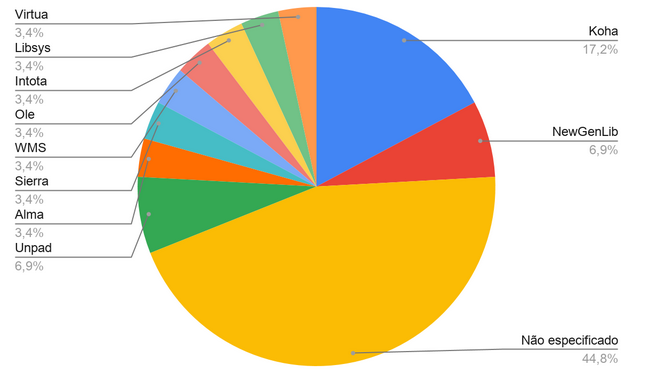
\includegraphics[width=.75\textwidth]{graph01.png}
\caption{Sistemas citados nos artigos encontrados}
\label{fig:exampleFig1}
\end{figure}
  \subsection{Quais as tendências de desenvolvimento relacionadas aos SGBs?}
  Uma análise das tecnologias e tendências em SGBs é explorado principalmente em \cite{7603363}. Segundo o estudo, existem 5 características dos futuros sistemas de gerenciamento:
  \begin{enumerate}
      \item Infraestrutura estável, separando as funções de banco de dados, interface do cliente e interface do servidor.
      \item Tem um back-end padronizado, pois estão passando a utilizar tecnologias de empresas com grande legado e influência no mercado.
      \item Os sistemas possuem diversas funções, como possuir módulos para museus ou bibliotecas de outros campus, se adaptando às necessidades de sua região.
      \item Os sistemas não precisam ser instalados pelos usuários, pois são oferecidos como um serviço.
      \item Utilização de computação em nuvem para  que qualquer atualização no sistema afete todos os usuários simultaneamente.
      \item Em adição à utilização dos sistemas como serviço de software, alguns sistemas devem ter módulos instalados localmente, como complemento, para o gerenciamento dos recursos digitais e físicos.
      \newline 
      \newline
Nas características principais, o estudo destaca:
      \item Ter uma API ou código aberto para que terceiros possam incrementar funcionalidades e adaptar o sistema às suas necessidades.
      \item Suporte a formatos e padrões relevantes, como catalogação de , recursos online, uso de estatística, uso de diversos padrões e formatos.
      \item Conhecimento centralizado para a reutilização de dados, relacionamento entre esses dados.
      \newline
      \newline
      Por fim, o estudo trata das tendências de desenvolvimento para SGBs, o que inclui:
\item Integração entre diferentes sistemas de gerenciamento;
\item Suporte para o novo padrão de descrição de recursos (RDA).
\item Integração com computação em nuvem.
\item Uso de dispositivos móveis.
\item Suporte a geração de conteúdo, compartilhamento de informação via blogs e redes sociais e participação de usuários.
  \end{enumerate}

\subsection{Quais as tecnologias embarcadas utilizadas nesses sistemas?}
Nessa questão de pesquisa, tratamos das tecnologias que não fazem parte dos SGBs, mas que são utilizados para melhorar processos nas bibliotecas ou melhorar alguns aspectos dos sistemas. No gráfico 2 são ilustradas as  tecnologias encontradas, com destaque para o uso de RFID e uso de dispositivos móveis. As tecnologias utilizadas e seus respectivos artigos estão tabelados na tabela 2.
\begin{table}[!!ht]
\centering
\textbf{\caption{Tecnologias por artigo.}}
\centering
\begin{tabular}{|c|c|}\hline
RFID  & \makecell{\cite{6632228}, \cite{7695207}, \\ \cite{liu2016design}, \cite{BAYANI2018}} \\ \hline
Nuvem & \cite{7603363}, \cite{Li2016MobileCB} \\ \hline
Tecnologias Móveis & \makecell{\cite{7603363}, \cite{Li2016MobileCB},\\ \cite{7695207}, \cite{7508166}}\\ \hline
Mineração de Dados & \cite{8525182} \\ \hline
Inteligência Artificial & \cite{8691086},\cite{7508166} \\ \hline
QR Code & \cite{8780424} \\ \hline
Blockchain & \cite{8805901} \\ \hline
Realidade Aumentada & \cite{7892686} \\ \hline
Realidade Virtual & \cite{8789229}\\ \hline
VRobótica & \cite{8473132}\\
\bottomrule
\end{tabular}
\label{tab:tecnologias}
\end{table}
A partir do gráfico 2, pode-se perceber uma predominância do uso de RFID e de tecnologias móveis, como tablets e smartphones. O uso de Inteligência Artificial e Computação em Nuvem também aparece como tecnologias mais emergentes, ainda não tão populares.
\begin{figure}[!!ht]
\centering
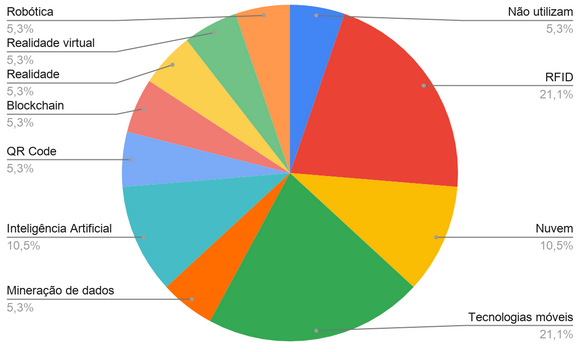
\includegraphics[width=.75\textwidth]{graph02.png}
\caption{Tecnologias utilizadas em conjunto com os SGBs}
\label{fig:exampleFig2}
\end{figure}
\section{Discussão e conclusão}
De acordo com os estudos considerados, vimos que os SGBs de código aberto estão entre os mais populares, como o Koha e o NewGenLib. Tal fato está em concordância com o estudo de \cite{7603363}, em que uma das tendências para o desenvolvimento dos SGBs contemporâneos e futuros é justamente ser de código aberto, de forma que possa se adaptar às necessidades particulares da biblioteca que faz uso de tal sistema. Outra tendência notada é o uso de dispositivos móveis como smartphones e tablets, trazendo facilidades para os usuários das bibliotecas. Do lado administrativo, predomina o uso de RFID, auxiliando na catalogação, organização e busca de exemplares. Também se destaca o uso de computação inteligente e computação em nuvem.

\bibliographystyle{sbc}
\bibliography{sbc-template}

\end{document}
